\chapter{AR Foundation}
\textbf{AR Foundation}\cite{AR-Foundation-1}\cite{AR-Foundation-2} è un package di Unity (il game engine su cui è sviluppata l'applicazione; un \textit{package} è un insieme di codice e risorse che si aggiunge a un progetto Unity) che espone un'unica API (Application Programming Interface, cioè l'insieme di classi e funzioni che lo sviluppatore può richiamare) per le funzionalità di realtà aumentata, come il tracciamento della posizione della camera, il rilevamento dei piani, i raycast e le ancore. È quindi un framework \textit{cross-platform}, ovvero un insieme di strumenti e librerie che permette di scrivere il codice una sola volta e ottenere app per più sistemi operativi, in questo caso Android e iOS (oltre ad alcuni visori AR/XR), senza modifiche al codice. AR Foundation, però, definisce soltanto \textit{che cosa} si può chiedere al sistema e non contiene l'implementazione di \textit{come} farlo. Per questo si comporta da regista: Unity organizza le funzionalità AR in \textit{subsystem} XR, interfacce generiche come quella dei piani, della camera o dei raycast, e il compito di realizzarle concretamente spetta ai \textbf{plug-in provider}, package separati da installare e abilitare per ciascuna piattaforma di destinazione: \textbf{ARCore XR Plugin} per Android e \textbf{ARKit XR Plugin} per iOS. Ogni plug-in implementa i subsystem di Unity e fa da traduttore, convertendo le richieste generiche di AR Foundation nelle chiamate dello SDK nativo della piattaforma. Uno \textit{SDK} (Software Development Kit) è un insieme di librerie, strumenti e documentazione fornito dal produttore di una tecnologia: su Android è l'\textbf{ARCore SDK} di Google, mentre su iOS è il framework \textbf{ARKit} di Apple. Il plug-in appartiene quindi a Unity, lo SDK a Google o Apple, e lo sviluppatore scrive codice solo con l'API di AR Foundation. Le funzioni specifiche di ARCore, come Geospatial e Cloud Anchors, richiedono invece un package a parte, \textbf{ARCore Extensions}.

Lo SDK ARCore, nella versione usata dal plug-in, è scritto in C/C++ ed è per questo che entra in gioco l'\textbf{NDK}\cite{NDK} (Native Development Kit), l'insieme di strumenti con cui Google permette di compilare per Android codice nativo, cioè codice C/C++ tradotto direttamente in istruzioni eseguibili dal processore del telefono. Il codice Java o Kotlin, invece, viene compilato in \textit{bytecode DEX} (un formato intermedio indipendente dal processore) ed eseguito da ART (Android Runtime), la macchina virtuale di Android; il codice nativo, non passando da questo livello, è più veloce e permette di riutilizzare librerie C/C++ già esistenti, per cui viene preferito per le parti più critiche come la visione artificiale. Il risultato della compilazione nativa sono le \textit{shared library}, file con estensione \texttt{.so} (shared object) che il sistema carica in memoria solo a runtime, cioè quando l'app è in esecuzione. Poiché ogni architettura di processore (ABI, ad esempio \texttt{arm64-v8a}) richiede la propria versione compilata, le librerie vengono collocate in cartelle separate per ABI. Lo stesso meccanismo riguarda Unity stesso: con lo scripting backend \textbf{IL2CPP}, il codice C\# dell'app viene convertito in C++ e compilato con l'NDK in una libreria \texttt{.so}. Durante la fase di \textit{build}, la compilazione e il confezionamento del progetto, tutte queste librerie (quelle di Unity, quelle del plug-in e quelle dello SDK ARCore) vengono inserite nell'\textbf{APK} (Android Package Kit), il file di installazione di un'app Android, equivalente all'\texttt{.exe} di Windows. Su iOS non esistono né NDK né file \texttt{.so}: il codice nativo viene compilato con Xcode in librerie statiche o framework.

Una volta installata l'app, il funzionamento a runtime segue una catena di chiamate che scende di livello a ogni passaggio. Quando uno script C\# invoca, ad esempio, \texttt{ARRaycastManager.Raycast} per capire quale superficie reale si trova sotto il punto toccato sullo schermo, AR Foundation inoltra la richiesta al subsystem corrispondente. Il provider di ARCore XR Plugin la raccoglie e, poiché il suo codice nativo è in C/C++, passa dal C\# alle funzioni delle librerie \texttt{.so} tramite \textit{P/Invoke} (Platform Invoke), il meccanismo di .NET per chiamare funzioni native. Queste librerie richiamano a loro volta l'API C dello SDK ARCore. Per le parti che invece vivono nel mondo Java, come la verifica dell'installazione di Google Play Services for AR o la richiesta dei permessi, si usa la \textbf{JNI} (Java Native Interface), il ponte che permette al codice nativo e a quello Java/Kotlin di chiamarsi a vicenda (in Unity spesso tramite \texttt{AndroidJavaObject}). Lo SDK, infine, non esegue da solo il tracciamento: comunica con il vero motore AR di sistema, \textbf{Google Play Services for AR}, un servizio separato dall'app che si installa e si aggiorna tramite Play Store, il quale analizza i frame della fotocamera e i dati dei sensori inerziali (accelerometro e giroscopio) per stimare la posizione del dispositivo e individuare i piani. Su iOS questo ruolo è svolto da ARKit, già integrato nel sistema operativo e quindi privo di installazione o aggiornamento separati. I risultati compiono poi il percorso inverso: il motore AR restituisce i dati allo SDK, il plug-in li converte nelle strutture generiche dei subsystem e AR Foundation li espone allo sviluppatore, ad esempio sotto forma di oggetti \texttt{ARPlane} aggiornati a ogni frame, permettendo di posizionare i contenuti virtuali sulla scena reale.



 \begin{center}
  Una lista di tutte le funzionalità che AR Foundation supporta:

    \begin{tabular}{| l | p{10cm} |}
      \hline
      \rowcolor{gray!30}
      \textbf{Caratteristica} & \textbf{Descrizione} \\ 
      \hline
      Sesssion & Attivare, disattivare e configurare la realtà aumentata sulla piattaforma di destinazione. \\ 
      \hline
      Device tracking & Tracciare la posizione e la rotazione del dispositivo nello spazio fisico. \\ 
      \hline
      Camera & Esegui il rendering delle immagini provenienti dalle fotocamere del dispositivo ed effettua la stima della luce \\ 
      \hline
      Plane Detection & Rileva e traccia le superfici piane. \\ 
      \hline
      Bounding Box Detection & Rileva e traccia i riquadri di delimitazione degli oggetti 3D. \\ 
      \hline
      Image Tracking & Rileva e traccia immagini 2D.\\ 
      \hline
      Markers & Traccia i marcatori AR e leggi i dati codificati in essi.\\ 
      \hline
      Object Tracking & Rileva e traccia oggetti 3D. \\ 
      \hline
      Face Tracking & Rilevare e tracciare i volti umani. \\ 
      \hline
      Body Tracking & Individuare e tracciare un corpo umano.\\ 
      \hline
      Point Clouds & Individua e traccia i punti caratteristici. \\ 
      \hline
      Ray Casts & Proietta raggi contro gli oggetti tracciati. \\
     \hline
      Anchors & Tracciare punti arbitrari nello spazio. \\
      \hline
      Meshing & Genera le mesh dell'ambiente.\\
      \hline
      Enviroment Probes & Genera mappe cubiche dell'ambiente. \\
      \hline
      Occlusion & Occulta i contenuti AR con oggetti fisici ed esegui la segmentazione umana. \\
      \hline
      Participants & Traccia altri dispositivi in una sessione AR condivisa. \\
      \hline
    \end{tabular}
\end{center}


\begin{center}
Non tutte le funzionalità sono supportate da tutte le piattaforme(Plug-in di Unity):

\begin{tabular}{| l | p{2cm} | p{2cm} |p{2cm} |}
      \hline
      \rowcolor{gray!30}
      \textbf{Caratteristica} & \textbf{Android} & \textbf{iOS} & \textbf{XR Sim.} \\ 
      \hline
      Sesssion & Si & Si & Si\\ 
      \hline
      Device tracking & Si & Si & Si \\ 
      \hline
      Camera & Si & Si & Si \\ 
      \hline
      Plane Detection & Si & Si & Si \\ 
      \hline
      Bounding Box Detection & & Si & Si\\ 
      \hline
      Image Tracking & Si & Si & Si\\ 
      \hline
      Markers &  & & \\ 
      \hline
      Object Tracking & & Si & \\ 
      \hline
      Face Tracking & Si & Si &\\ 
      \hline
      Body Tracking & & Si & \\ 
      \hline
      Point Clouds & Si & Si & Si\\ 
      \hline
      Ray Casts & Si & Si & Si \\
     \hline
      Anchors & Si & Si & Si \\
      \hline
      Meshing &  & Si & Si\\
      \hline
      Enviroment Probes & Si & Si & Si\\
      \hline
      Occlusion & Si & Si & Si\\
      \hline
      Participants &  & Si & \\
      \hline
    \end{tabular}
\end{center}

 \subsection{Architettura}
 
L'architettura di Unity AR Foundation \cite{AR-Foundation-1} si basa su tre concetti fondamentali, pensati per astrarre le differenze tra gli SDK nativi di realtà aumentata: \textbf{Subsystems}, \textbf{Managers} ed \textbf{Extensions}. 

 \begin{figure}[H]
            \centering
            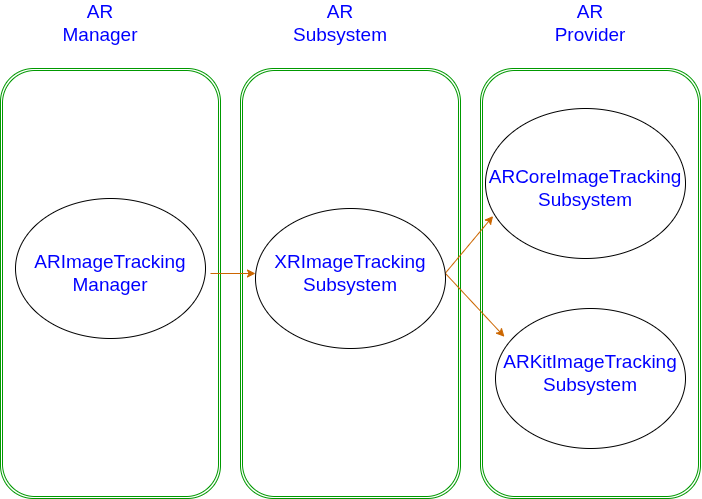
\includegraphics[width=0.8\textwidth]{images/ar-foundation/AR-Working.png} 
            \caption{AR Foundation Workflow (Example Feature: Image Tracking)}
            \label{fig:dt}
    \end{figure}

La figura mostra come collaborano i diversi livelli per una funzionalità di esempio, il tracciamento di immagini.
Al livello più alto si trova \texttt{ARTrackedImageManager}, un componente (\texttt{MonoBehaviour}) che lo sviluppatore aggiunge al GameObject \texttt{XR Origin} della scena. Serve a gestire gli eventi e ad accedere alle immagini tracciate, e permette di assegnare una \textit{Reference Image Library} (la lista di immagini da riconoscere) e un \textit{Prefab} da istanziare sopra l'immagine quando viene rilevata.
Al livello intermedio si trova \texttt{XRImageTrackingSubsystem}, il sottosistema che definisce l'interfaccia standard di Unity per il tracciamento di immagini, indipendente dal dispositivo. Stabilisce le regole e i metodi che ogni piattaforma (Android, iOS, ecc.) deve implementare, garantendo così il principio cross-platform.
Al livello più basso si trova il provider specifico della piattaforma, ovvero l'implementazione concreta fornita dal plug-in: ARCore XR Plugin su Android, ARKit XR Plugin su iOS. Il provider traduce i comandi generici del sottosistema in chiamate allo SDK nativo, che comunica con gli algoritmi di visione artificiale di ARCore per riconoscere, attraverso la fotocamera, i punti caratteristici (\textit{feature points}) dell'immagine di riferimento. Quando l'app viene compilata per Android, Unity attiva automaticamente il provider corrispondente.

\subsubsection{Subsystems}
Un \textbf{sottosistema}, implementato in Unity tramite la classe base \texttt{SubsystemWithProvider} \cite{AR-Foundation-1}, definisce il ciclo di vita e l'interfaccia di scripting di una specifica funzionalità del motore. Ad esempio, \texttt{XRPlaneSubsystem} definisce l'interfaccia di tracciamento dei piani: lo stesso codice applicativo può usare un piano rilevato sia su iOS sia su Android, perché AR Foundation non contiene le implementazioni a basso livello. Queste sono fornite dai \textbf{provider}, distribuiti in pacchetti detti \textbf{plug-in provider} (\textit{Google ARCore XR} per Android, \textit{Apple ARKit XR} per iOS), e costituiscono il livello di astrazione tra il codice applicativo e gli SDK proprietari.

Tutti i sottosistemi condividono lo stesso ciclo di vita (creazione, avvio, arresto, distruzione), gestito dall'\texttt{XRLoader} attivo nel progetto: ogni plug-in provider include il proprio loader, che istanzia i sottosistemi all'avvio dell'app e li distrugge alla chiusura (configurabile da \textit{Project Settings $>$ XR Plug-in Management}).

Ogni sottosistema ha un \textbf{descrittore} (\texttt{SubsystemDescriptor}) che indica le funzionalità supportate. Poiché queste dipendono da hardware e SDK, vanno verificate a runtime prima dell'uso:

\begin{lstlisting}[language={[Sharp]C}]
var trackedImageManager = FindFirstObjectByType<ARTrackedImageManager>();

// Il provider supporta la modifica a runtime della libreria immagini?
if (trackedImageManager.descriptor.supportsMutableLibrary)
{
    // Logica specifica per librerie dinamiche
}
\end{lstlisting}

I \textbf{sottosistemi di tracciamento} rilevano e seguono entità fisiche dell'ambiente dette \textbf{trackable} (ad esempio \texttt{XRPlaneSubsystem} rileva i \texttt{BoundedPlane}). Ogni trackable ha un \textbf{TrackableId}, un GUID (Globally Unique Identifier) a 128 bit che lo identifica in modo univoco, durante la sessione AR, nelle fasi di aggiunta, aggiornamento e rimozione. In \texttt{UnityEngine.XR.ARSubsystems} i trackable sono \texttt{struct} ad alte prestazioni che implementano \texttt{ITrackable}; in \texttt{UnityEngine.XR.ARFoundation} sono invece componenti \texttt{MonoBehaviour} (es. \texttt{ARPlane}) che le incapsulano.

\subsubsection{Managers}
Un \textbf{Manager} è un componente Unity (\texttt{MonoBehaviour}) che espone un'interfaccia ad alto livello per configurare una specifica funzionalità AR (piani, immagini tracciate, volti). I Manager ereditano da \texttt{SubsystemLifecycleManager} e fanno da ponte tra i dati dei sottosistemi XR e gli oggetti della scena, sincronizzandone il ciclo di vita con quello del componente: in \texttt{OnEnable} invocano \texttt{Start()} sul sottosistema associato, in \texttt{OnDisable} invocano \texttt{Stop()}.

I \textit{Trackable Manager} (\texttt{ARPlaneManager}, \texttt{ARTrackedImageManager}, ...) creano, aggiornano e distruggono automaticamente i \texttt{GameObject} dei trackable, istanziandoli come figli di \texttt{XR Origin} e posizionandoli rispetto al suo spazio di riferimento. Si può assegnare un \textit{Prefab} per la loro rappresentazione visiva (ad esempio una mesh per un piano); se manca, il Manager crea un \texttt{GameObject} vuoto con il componente \texttt{ARTrackable} idoneo, che aggiunge a runtime anche a un Prefab che ne fosse privo.

\subsubsection{Extensions}
AR Foundation non espone tramite astrazioni C\# tutte le API dei singoli SDK nativi. Per colmare il divario fornisce puntatori nativi grezzi (\texttt{nativePtr}), che permettono di accedere direttamente alle strutture del provider; ad esempio, \texttt{XRSessionSubsystem} espone la proprietà \texttt{nativePtr}. Struttura e indirizzo sono definiti da ciascun plug-in provider: per convenzione il puntatore indirizza una struttura il cui primo membro è un intero con la versione dell'interfaccia, seguito dai puntatori grezzi.

\begin{lstlisting}[language=C]
typedef struct UnityXRNativeSessionPtr
{
    int version;
    void* session;
} UnityXRNativeSessionPtr;
\end{lstlisting}

A causa dell'allineamento in memoria (\textit{struct padding}), \texttt{session} non si trova necessariamente a 4 byte dall'inizio: su architetture a 64 bit l'offset può essere di 8 byte. Quasi tutti i trackable (piani, immagini, volti) espongono un puntatore nativo; tramite chiamate P/Invoke è così possibile recuperare oggetti interni della piattaforma, come \texttt{ARFrame}, la sessione nativa (\texttt{ARSession} su iOS, \texttt{ArSession} su Android) e gli elementi geometrici dell'ambiente.



\subsection{Componenti Principali}
AR Foundation\cite{AR-Foundation-3} prevede l'uso di alcuni concetti fondamentali, i quali sono comuni a tutte le AR App.

\subsubsection{AR Session}
Il GameObject AR Session gestisce lo stato del dispositivo AR e la sessione corrente: quando tutti i componenti sono inizializzati e funzionano correttamente, lo stato assume il valore di \textit{SessionTracking}. Questo componente controlla l'intero ciclo di vita dell'esperienza di realtà aumentata.
Contiene inoltre lo script AR Input Manager, fondamentale per abilitare il tracciamento dello spazio circostante.

\subsubsection{XR Origin}
Il GameObject XR Origin converte i dati di tracciamento del dispositivo (come punti di interesse o piani detected) nello spazio coordinate di Unity. Ciò garantisce che la scena virtuale sia perfettamente sincronizzata con il mondo reale e ospita al suo interno la AR Camera.
Mentre gli elementi tracciabili vengono gestiti dal dispositivo nello "spazio sessione" (relativo al sistema di coordinate locale del dispositivo), i GameObject in Unity vengono posizionati nello "spazio mondo".

\subsubsection{Tracked Pose Driver (InputSystem)}
Il Tracked Pose Driver è un componente applicato alla fotocamera AR che ne aggiorna la posizione e la rotazione locali in tempo reale, basandosi sulle informazioni di tracciamento fornite dal sensore/dispositivo.

\subsubsection{AR Camera Manager}
L'AR Camera Manager gestisce il flusso video della fotocamera principale del dispositivo, combinando lo sfondo reale con gli elementi grafici 3D virtuali. Attraverso questo script è possibile configurare l'autofocus (di norma consigliato attivo, tranne nei contesti di inquadratura esclusivamente a lunga distanza).
Consente inoltre di attivare la stima della luminosità (light estimation) per aggiornare la sorgente di luce della scena Unity e di effettuare lo switch tra la fotocamera posteriore e quella frontale.


\subsection{Perché AR Foundation?}

Sviluppare applicazioni AR mobile con gli SDK nativi comporta costi di produzione più alti, scarsa portabilità del codice e una gestione degli aggiornamenti separata per ogni piattaforma. Uno \textbf{SDK} (Software Development Kit)\cite{SDK} è un insieme di strumenti forniti dal produttore di una piattaforma per sviluppare software per essa: compilatore, librerie con un'interfaccia pubblica detta \textbf{API} (Application Programming Interface), che permette a software diversi di comunicare, documentazione e informazioni sulle licenze di distribuzione. Gli SDK sono quindi specifici per un ecosistema: nel caso della realtà aumentata, \textbf{ARKit} di Apple funziona solo su iOS e \textbf{ARCore} di Google solo su Android, e il codice scritto per uno non è riutilizzabile sull'altro. AR Foundation nasce proprio per \textbf{evitare di scrivere e mantenere due codici diversi per la stessa funzione}, introducendo un livello di astrazione che traduce le istruzioni verso i rispettivi SDK.

\begin{figure}[H]
    \centering
    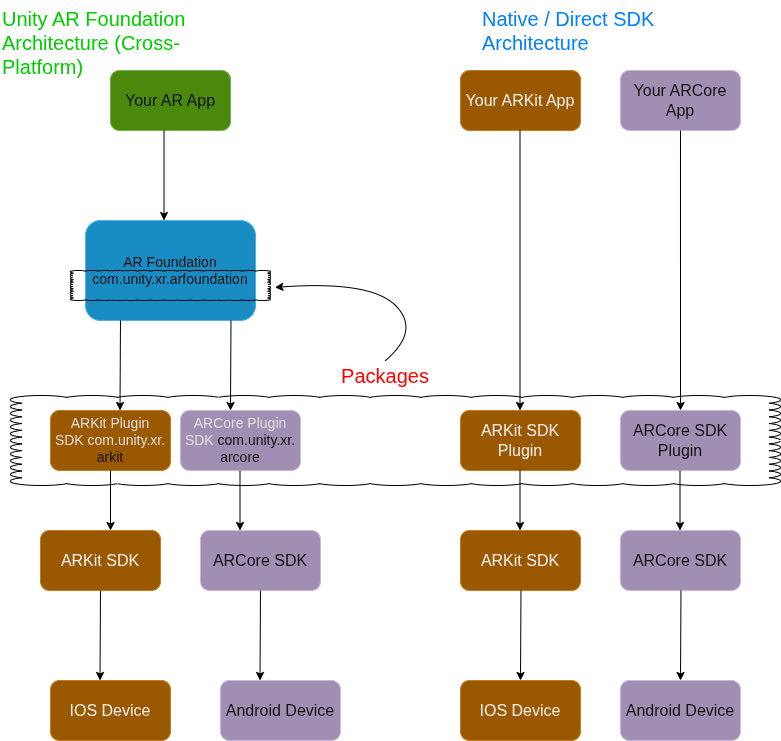
\includegraphics[width=0.9\textwidth]{images/ar-foundation/AR-Architecture.png}
    \caption{AR Foundation Architecture vs Native Architecture}
    \label{fig:ar-architecture}
\end{figure}

\begin{itemize}
    \item \textbf{ARKit XR Plugin (\texttt{com.unity.xr.arkit})} e \textbf{ARCore XR Plugin (\texttt{com.unity.xr.arcore})}: package Unity ufficiali, gestiti tramite lo Unity Package Manager (UPM). Agiscono da \textit{provider} nell'architettura XR di Unity: contengono codice C\# e librerie native (\texttt{.a} per iOS, \texttt{.so} per Android) che fanno da ponte tra l'interfaccia astratta di AR Foundation e l'SDK nativo.

    \item \textbf{ARKit e ARCore (SDK nativi)}: non sono package Unity, ma i framework forniti da Apple e Google. Eseguono il tracciamento e la visione artificiale a basso livello: ARKit è integrato nel sistema operativo, mentre ARCore si appoggia al servizio di sistema Google Play Services for AR.

    \item \textbf{Accesso diretto alle funzioni native}: AR Foundation non funziona da sola, ma sempre tramite i provider. Per funzioni esclusive non ancora astratte, lo sviluppatore può usare le API esposte dai plug-in (ad esempio \texttt{ARKitSessionSubsystem} o \texttt{ARCoreSessionSubsystem}) senza scrivere plug-in C/C++ personalizzati. Per ARCore, funzioni come Geospatial e Cloud Anchors richiedono il package aggiuntivo \textbf{ARCore Extensions}.
\end{itemize}

Il vantaggio principale di AR Foundation è lo sviluppo con un'unica base di codice (\textit{single codebase}) valida sia per iOS sia per Android, che riduce tempi di sviluppo, manutenzione e costi di produzione. A ciò si aggiungono la rapidità di prototipazione, grazie alla configurazione dei componenti direttamente nell'editor di Unity, e l'integrazione nativa con l'ecosistema Unity: pipeline di rendering, profiler, sistema UI e Visual Scripting.

Gli svantaggi sono due. Il primo è che le novità hardware e le nuove API di Google o Apple non sono disponibili subito: bisogna attendere che Unity le supporti, e un ritardo in un aggiornamento o in un bugfix può bloccare il progetto. Il secondo è che il livello di astrazione introduce un overhead, con un impatto (generalmente contenuto) su framerate e uso di CPU e RAM.

L'approccio nativo con ARCore, privo di livelli intermedi, offre invece le massime prestazioni, un consumo di risorse minore, accesso immediato alle ultime funzionalità e integrazione profonda con i servizi della piattaforma, oltre all'accesso di basso livello a sensori, fotocamera e memoria. Il prezzo è però elevato: una curva di apprendimento più ripida, codice più verboso (\textit{boilerplate}), competenze specifiche per ciascuna piattaforma e una doppia manutenzione. Un'app con ARCore nativo funziona solo su Android, e per coprire iOS bisogna riscrivere la logica con ARKit, mantenendo due basi di codice da aggiornare e testare nel tempo.